%%%%%%%%%%%%%%%%%%%%%%%%%%%%%%%%%%%%%%%%%
% Short Sectioned Assignment LaTeX Template Version 1.0 (5/5/12)
% This template has been downloaded from: http://www.LaTeXTemplates.com
% Original author:  Frits Wenneker (http://www.howtotex.com)
% License: CC BY-NC-SA 3.0 (http://creativecommons.org/licenses/by-nc-sa/3.0/)
%%%%%%%%%%%%%%%%%%%%%%%%%%%%%%%%%%%%%%%%%

%----------------------------------------------------------------------------------------
%	PACKAGES AND OTHER DOCUMENT CONFIGURATIONS
%----------------------------------------------------------------------------------------

\documentclass[paper=a4, fontsize=11pt]{scrartcl} % A4 paper and 11pt font size

% ---- Entrada y salida de texto -----

\usepackage{array}
\usepackage{booktabs}
\usepackage{tabulary}
\usepackage{multirow}

\usepackage{color}
\usepackage{listings}
\usepackage[T1]{fontenc} % Use 8-bit encoding that has 256 glyphs
\usepackage[utf8]{inputenc}
%\usepackage{fourier} % Use the Adobe Utopia font for the document - comment this line to return to the LaTeX default
\usepackage{footnote}
\usepackage{eurosym}
\usepackage{eurosym} % Sirve para poner \euro y que salga el símbolo del €.

% ---- Idioma --------
 
\usepackage[spanish, es-tabla]{babel} % Selecciona el español para palabras introducidas automáticamente, p.ej. "septiembre" en la fecha y especifica que se use la palabra Tabla en vez de Cuadro

% ---- Otros paquetes ----
\usepackage{subfig}
\usepackage{url} % ,href} %para incluir URLs e hipervínculos dentro del texto (aunque hay que instalar href)
\usepackage{amsmath,amsfonts,amsthm} % Math packages
%\usepackage{graphics,graphicx, floatrow} %para incluir imágenes y notas en las imágenes
\usepackage{graphics,graphicx, float} %para incluir imágenes y colocarlas

% Para hacer tablas comlejas
%\usepackage{multirow}
%\usepackage{threeparttable}

%\usepackage{sectsty} % Allows customizing section commands
%\allsectionsfont{\centering \normalfont\scshape} % Make all sections centered, the default font and small caps

\usepackage{fancyhdr} % Custom headers and footers
\pagestyle{fancyplain} % Makes all pages in the document conform to the custom headers and footers
\fancyhead{} % No page header - if you want one, create it in the same way as the footers below
\fancyfoot[L]{} % Empty left footer
\fancyfoot[C]{} % Empty center footer
\fancyfoot[R]{\thepage} % Page numbering for right footer
\renewcommand{\headrulewidth}{0pt} % Remove header underlines
\renewcommand{\footrulewidth}{0pt} % Remove footer underlines
\setlength{\headheight}{13.6pt} % Customize the height of the header

\numberwithin{equation}{section} % Number equations within sections (i.e. 1.1, 1.2, 2.1, 2.2 instead of 1, 2, 3, 4)
\numberwithin{figure}{section} % Number figures within sections (i.e. 1.1, 1.2, 2.1, 2.2 instead of 1, 2, 3, 4)
\numberwithin{table}{section} % Number tables within sections (i.e. 1.1, 1.2, 2.1, 2.2 instead of 1, 2, 3, 4)

\setlength\parindent{0pt} % Removes all indentation from paragraphs - comment this line for an assignment with lots of text

\newcommand{\horrule}[1]{\rule{\linewidth}{#1}} % Create horizontal rule command with 1 argument of height


\title{	
	\normalfont \normalsize 
	\textsc{\textbf{Inteligencia de Negocio (2017-2018)} \\ Grado en Ingeniería Informática \\ Universidad de Granada} \\ [25pt] 
	\horrule{0.5pt} \\[0.4cm]
	\huge Práctica 2 \\
	\horrule{2pt} \\[0.5cm]
}

\author{Juan José Sierra González \\ jjsierra103@gmail.com}

\date{\normalsize\today}

\begin{document}
	\maketitle
	\thispagestyle{empty}
	
	\newpage
	
	\tableofcontents
	
	\listoffigures
	
	\listoftables
	
	\newpage
	
	\section{Introducción}
	En esta práctica se tratará de interpretar el comportamiento de distintos algoritmos de clustering, trabajando sobre una base de datos de accidentes en España en el año 2013. Eligiendo distintos subconjuntos del conjunto total de datos se elaborarán 3 casos de estudio sobre los que ejecutar los algoritmos. Estos algoritmos de clustering seleccionados para el estudio son \textbf{K-Means, DBSCAN, Spectral Clustering, Birch y Ward}.\\
	
	Para cada caso de estudio se mostrarán las tablas de resultados y algunas gráficas ilustrativas y se tratará de dar la visión e interpretación más adecuada de las mismas.
	
	\section{Caso de estudio 1}
	
	\subsection{¿Qué se analiza?}
	En el primero de estos casos de estudio se van a analizar los \textbf{accidentes que han tenido lugar en autovías y autopistas}. Las características seleccionadas para el estudio han sido el número de vehículos implicados, el número de heridos graves y leves, el número de fallecidos y el total de víctimas afectadas. Se comprobará cuántos vehículos suelen verse involucrados en estos accidentes y cómo se distribuyen las cifras de heridos y víctimas mortales, es decir, tratar de valorar si la cifra de fallecidos en accidentes de este ámbito representa un dato sustancial frente al total de accidentes o son una pequeña muestra dentro de los accidentes registrados.\\
	
	Este caso de estudio en cuestión cuenta con 11943 ejemplos. Es el más vasto de los que se van a estudiar,
	
	\subsection{Resultados de los algoritmos}
	En este correspondiente apartado para cada caso de estudio se mostrará una tabla que recoja algunos resultados analíticos del comportamiento de los distintos algoritmos de clustering sobre el subconjunto de datos que representa el caso de estudio. En la tabla se incluyen el número de clusters en los que el algoritmo ha segmentado los ejemplos, el tiempo de ejecución y los scores obtenidos según las métricas de Calinski-Harabaz y Silhouette (estos no son calculados para el algoritmo de clustering jerárquico del estudio, el Ward). Además, para cada caso de estudio se han realizado unos filtros a los clusters, para que aquellos que tienen menos de un determinado número pequeño de ejemplos no se consideren representativos y no formen parte de los cómputos de las matrices de dispersión y los mapas de calor. En la tabla se incluyen el número de clusters que ha quedado después del filtrado y el número de ejemplos que se encontraban dentro de los clusters eliminados.\\
	
	Puesto que contaremos con un número de ejemplos muy variado entre casos de estudio, el criterio que he seguido para el filtrado de los clusters ha sido el siguiente:
	\begin{itemize}
		\item Si el conjunto de datos tiene más de 100 ejemplos, eliminar aquellos clusters que no representen el 1\% de la población.
		\item Si el conjunto de datos no supera los 100 ejemplos, eliminar aquellos clusters que representan 2 ejemplos o menos.
	\end{itemize}

	A continuación se muestra la tabla de resultados del primer caso de estudio.
	
	\begin{table}[H]
		\centering
		\resizebox{\textwidth}{!}{
			$\begin{tabular}{ *{7}{c} }
			\toprule
			\textbf{Algorithm} & \textbf{Clusters} & \textbf{Execution time} & \textbf{CH Score} & \textbf{Silhouette Score} & \textbf{Clusters after filtering} & \textbf{Number of samples dropped}\\
			\midrule
			K-Means & 4 & 0.349 & 17443.397 & 0.74487 & 4 & 0 \\			
			DBSCAN & 26 & 0.895 & 322.707 & 0.31788 & 3 & 530 \\			
			Birch & 4 & 0.374 & 10526.549 & 0.67967 & 3 & 91 \\			
			Spectral Clustering & 4 & 53.784 & 13864.674 & 0.71842 & 4 & 0 \\			
			Ward & 100 & 3.251 & - & - & 10 & 1186 \\
			\bottomrule
			\end{tabular}$
		}
		\caption{Resultados de los algoritmos de clustering para el primer caso de estudio.}
		\label{tablaTodos1}
	\end{table}

	En primer lugar será necesario explicar qué representan las métricas Calinski-Harabaz y Silhouette, para poder realizar un análisis suficientemente explicativo.\\
	
	La métrica \textbf{Calinski-Harabaz} valora para cada algoritmo la similitud entre los ejemplos dentro de un mismo cluster y la diferenciación con el resto de clusters. Dicho de otra forma, refleja un valor real que es mejor cuanta mayor similitud haya intra-cluster y menor haya entre-cluster. A mayor valor Calinski-Harabaz, mejor separados están los ejemplos de la población para k-clusters.\\
	
	La métrica \textbf{Silhouette} valora en cierto modo la misma situación que el Calinski-Harabaz, pero tratando especialmente la distancia que hay entre el ejemplo más lejano del mismo cluster y el ejemplo más cercano de un cluster diferente. En este caso se obtendrá una valoración Silhouette que siempre estará en el intervalo [-1,1], y que a mayor valor indica una mejor distribución de los ejemplos entre los clusters.\\

	Para cada caso de estudio se centrará el análisis sobre un par de algoritmos, para no extender demasiado el contenido de la memoria. Para estos algoritmos se mostrarán una matriz de dispersión y un mapa de calor (\textit{heatmap}).\\

	De acuerdo a lo explicado y viendo los resultados de la tabla anterior, parece que los algoritmos que mejor separan los ejemplos en clusters son el K-Means y el Spectral Clustering, y además se observa que existe una relación casi proporcional entre las dos métricas. Sin embargo como K-Means y Spectral Clustering representan los ejemplos en el mismo número de clusters y sin filtrar nada, no veo tan interesante analizar ambos, y voy a analizar \textbf{K-Means} y \textbf{Birch}, que realizando un filtrado de un cluster obtiene una valoración relativamente buena, para ver cómo es capaz de dividir los ejemplos.

	\subsubsection{K-Means}
	En primer lugar se incluye la matriz de dispersión del algortimo K-Means.
	
	\begin{figure}[H]
		\centering
		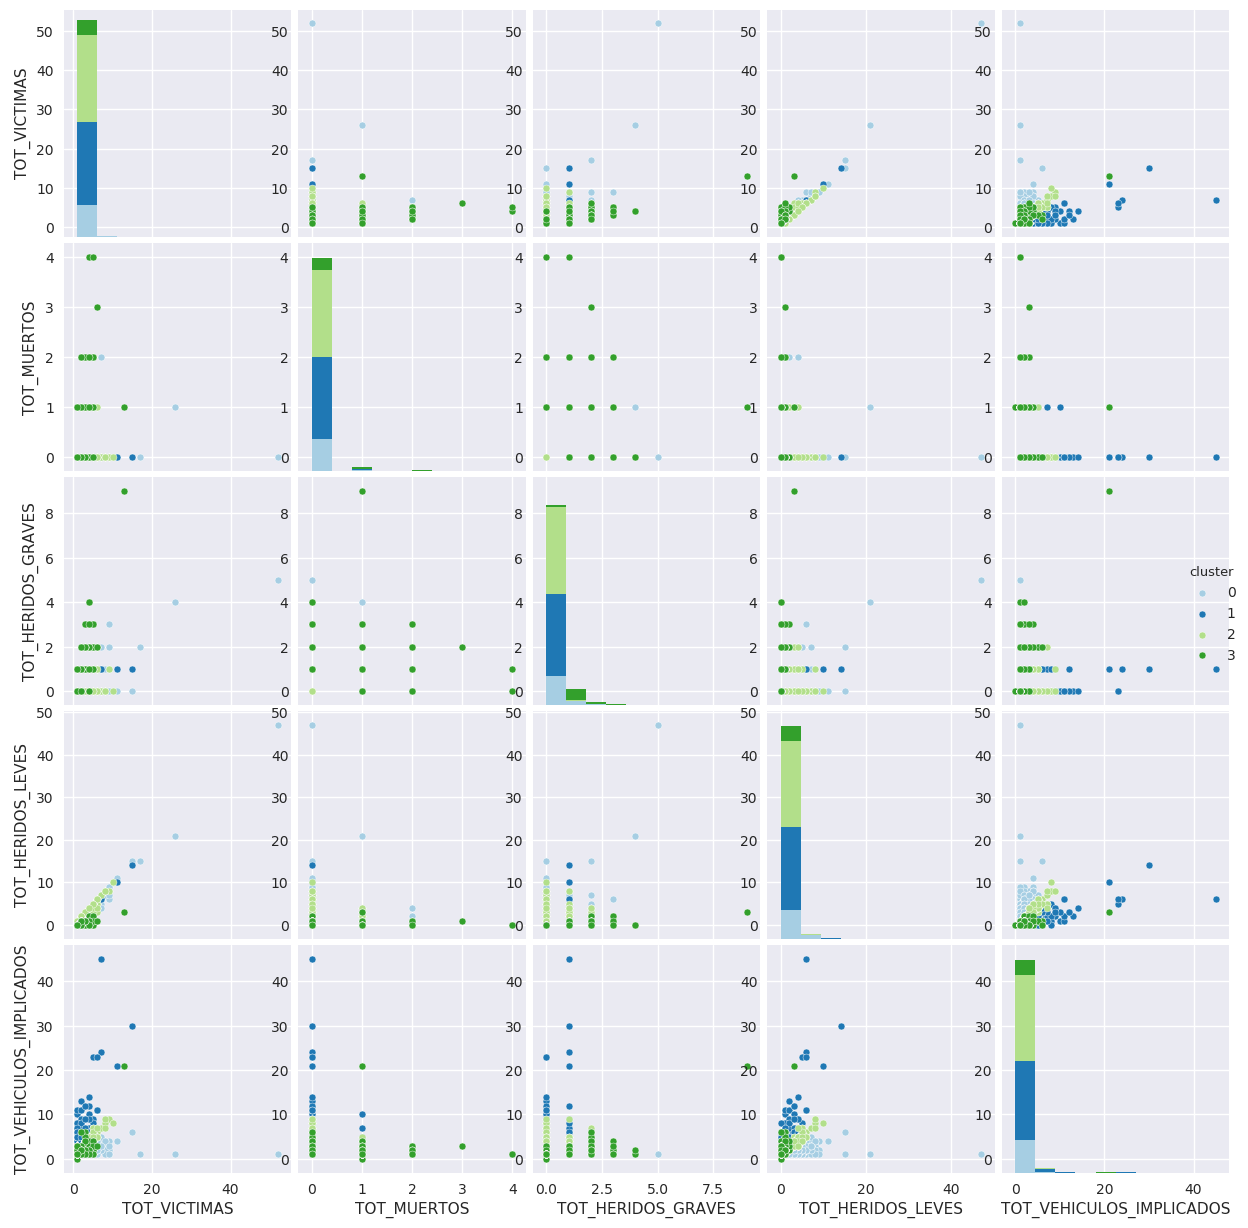
\includegraphics[scale=0.5]{plots/K-Means-HighwayAccidents-ScatterMatrix.png}
		\caption{Matriz de dispersión del algoritmo K-Means para el primer caso de estudio.}
	\end{figure}

	Para ayudar a la interpretación de la matriz de dispersión se ha incluido una tabla que comprende los valores medios de cada variable a estudiar para cada uno de los clusters que han quedado tras el filtrado, que son los mismos que se muestran en la gráfica anterior.

	\begin{table}[H]
		\centering
		\resizebox{\textwidth}{!}{
			\begin{tabular}{*{6}{c}}
				\toprule
				\textbf{CLUSTER} &  \textbf{TOT\_HERIDOS\_GRAVES} &  \textbf{TOT\_HERIDOS\_LEVES} &  \textbf{TOT\_MUERTOS} &  \textbf{TOT\_VEHICULOS\_IMPLICADOS} &  \textbf{TOT\_VICTIMAS} \\
				\midrule
				\textbf{0} &            0.140774 &           2.958497 &     0.018508 &                  1.453730 &      3.117779 \\
				\textbf{1} &            0.009233 &           1.143548 &     0.013410 &                  2.563860 &      1.166190 \\
				\textbf{2} &            0.005417 &           1.444375 &     0.003333 &                  1.451667 &      1.453125 \\
				\textbf{3} &            1.039457 &           0.146732 &     0.209618 &                  1.579531 &      1.395808 \\
				\bottomrule
			\end{tabular}
		}
		\caption{Tabla de valores medios del algoritmo K-Means para el primer caso de estudio.}
	\end{table}
	
	Por último, también se incluye un heatmap para mostrar cómo se distribuyen los valores de cada variable entre los clusters de una forma más ilustrativa. En este caso se representan los clusters contra las variables, y en cada casilla aparece el valor medio normalizado para dicha variable.
	
	\begin{figure}[H]
		\centering
		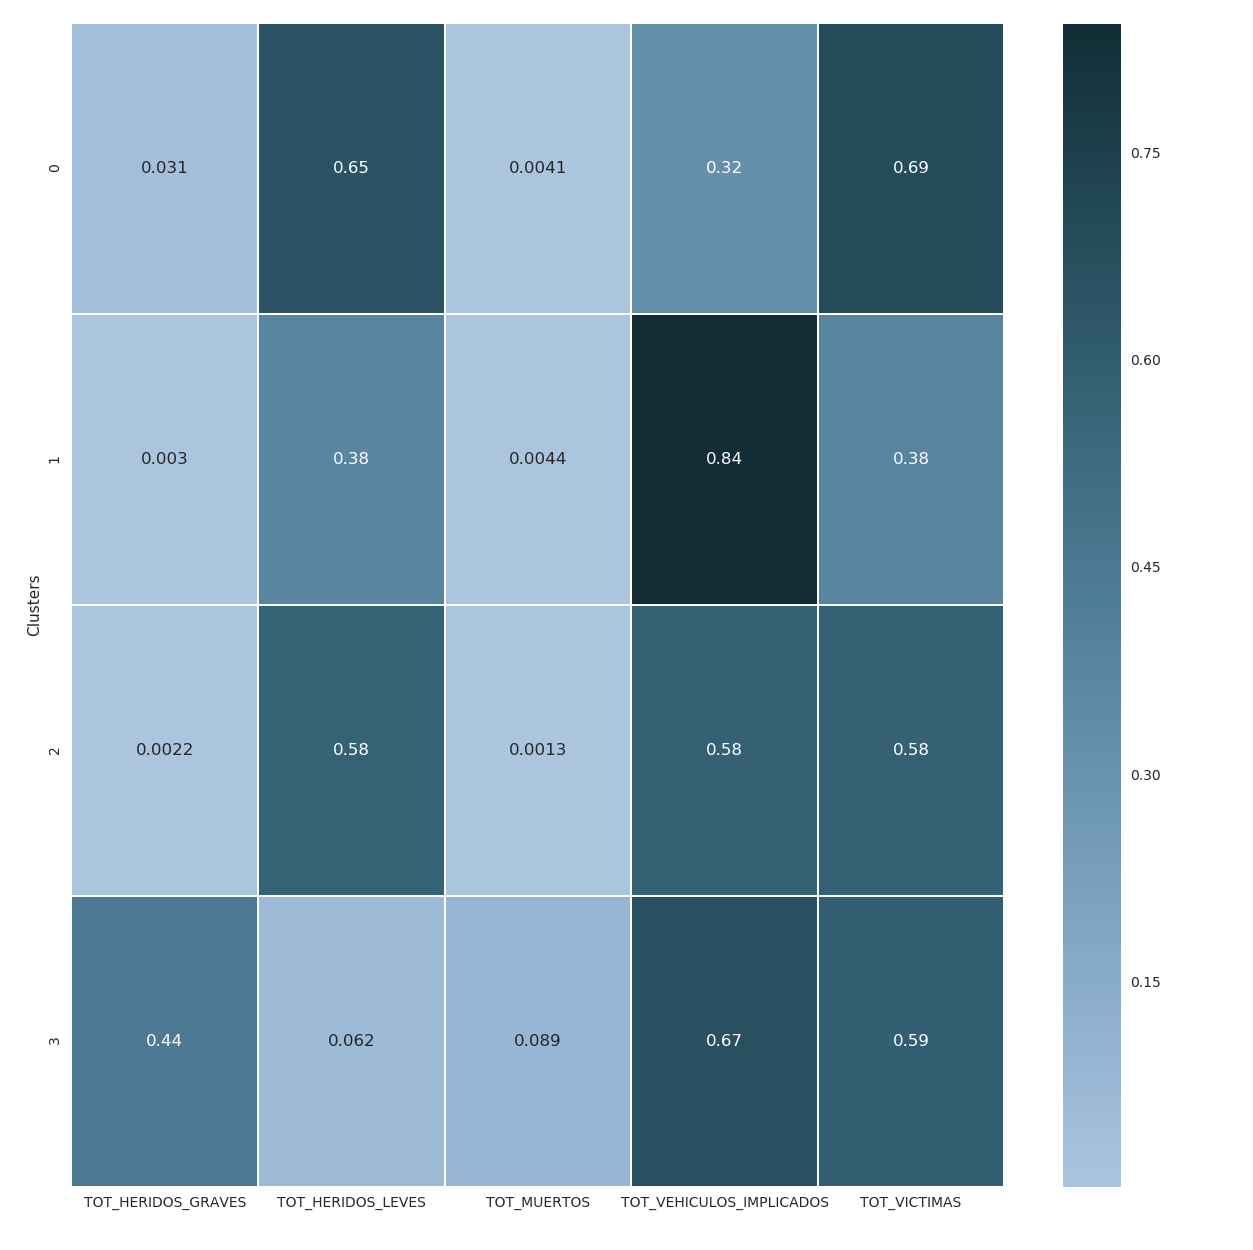
\includegraphics[scale=0.4]{heatmaps/K-Means-HighwayAccidents-Heatmap.png}
		\caption{Heatmap del algoritmo K-Means para el primer caso de estudio.}
	\end{figure}

	\subsubsection{Birch}
	A continuación se incluye la matriz de dispersión del algoritmo Birch para este primer caso de estudio.
	
	\begin{figure}[H]
		\centering
		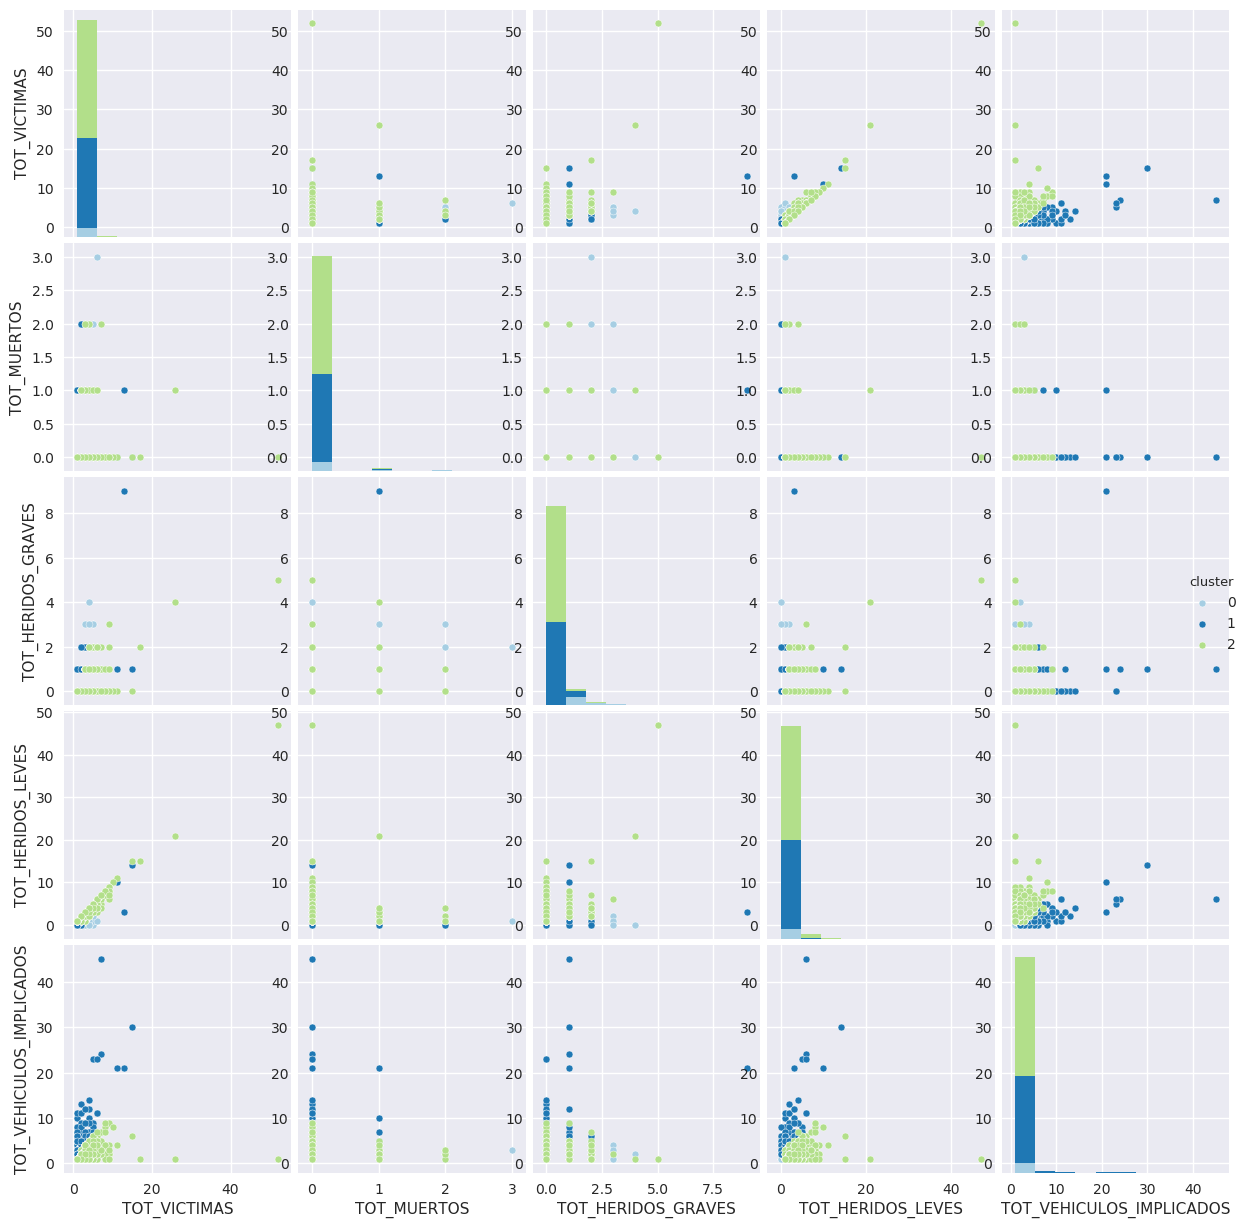
\includegraphics[scale=0.5]{plots/Birch-HighwayAccidents-ScatterMatrix.png}
		\caption{Matriz de dispersión del algoritmo Birch para el primer caso de estudio.}
	\end{figure}

	Ahora se muestra la tabla de valores medios por variable para cada cluster dentro de este caso de estudio.
	
	\begin{table}[H]
		\centering
		\resizebox{\textwidth}{!}{
			\begin{tabular}{*{6}{c}}
				\toprule
				\textbf{CLUSTER} &  \textbf{TOT\_HERIDOS\_GRAVES} &  \textbf{TOT\_HERIDOS\_LEVES} &  \textbf{TOT\_MUERTOS} &  \textbf{TOT\_VEHICULOS\_IMPLICADOS} &  \textbf{TOT\_VICTIMAS} \\
				\midrule
				\textbf{0} &            1.216433 &           0.278557 &     0.124248 &                  1.166333 &      1.619238 \\
				\textbf{1} &            0.077951 &           1.089264 &     0.012341 &                  2.545455 &      1.179556 \\
				\textbf{2} &            0.026960 &           1.863195 &     0.007857 &                  1.456632 &      1.898013 \\
				\bottomrule
			\end{tabular}
		}
		\caption{Tabla de valores medios del algoritmo K-Means para el primer caso de estudio.}
	\end{table}

	Y por último, también se muestra el heatmap que representa el valor medio normalizado por cada variable para cada uno de los clusters, para ayudar a visualizar la tabla anterior de forma más clara.

	\begin{figure}[H]
		\centering
		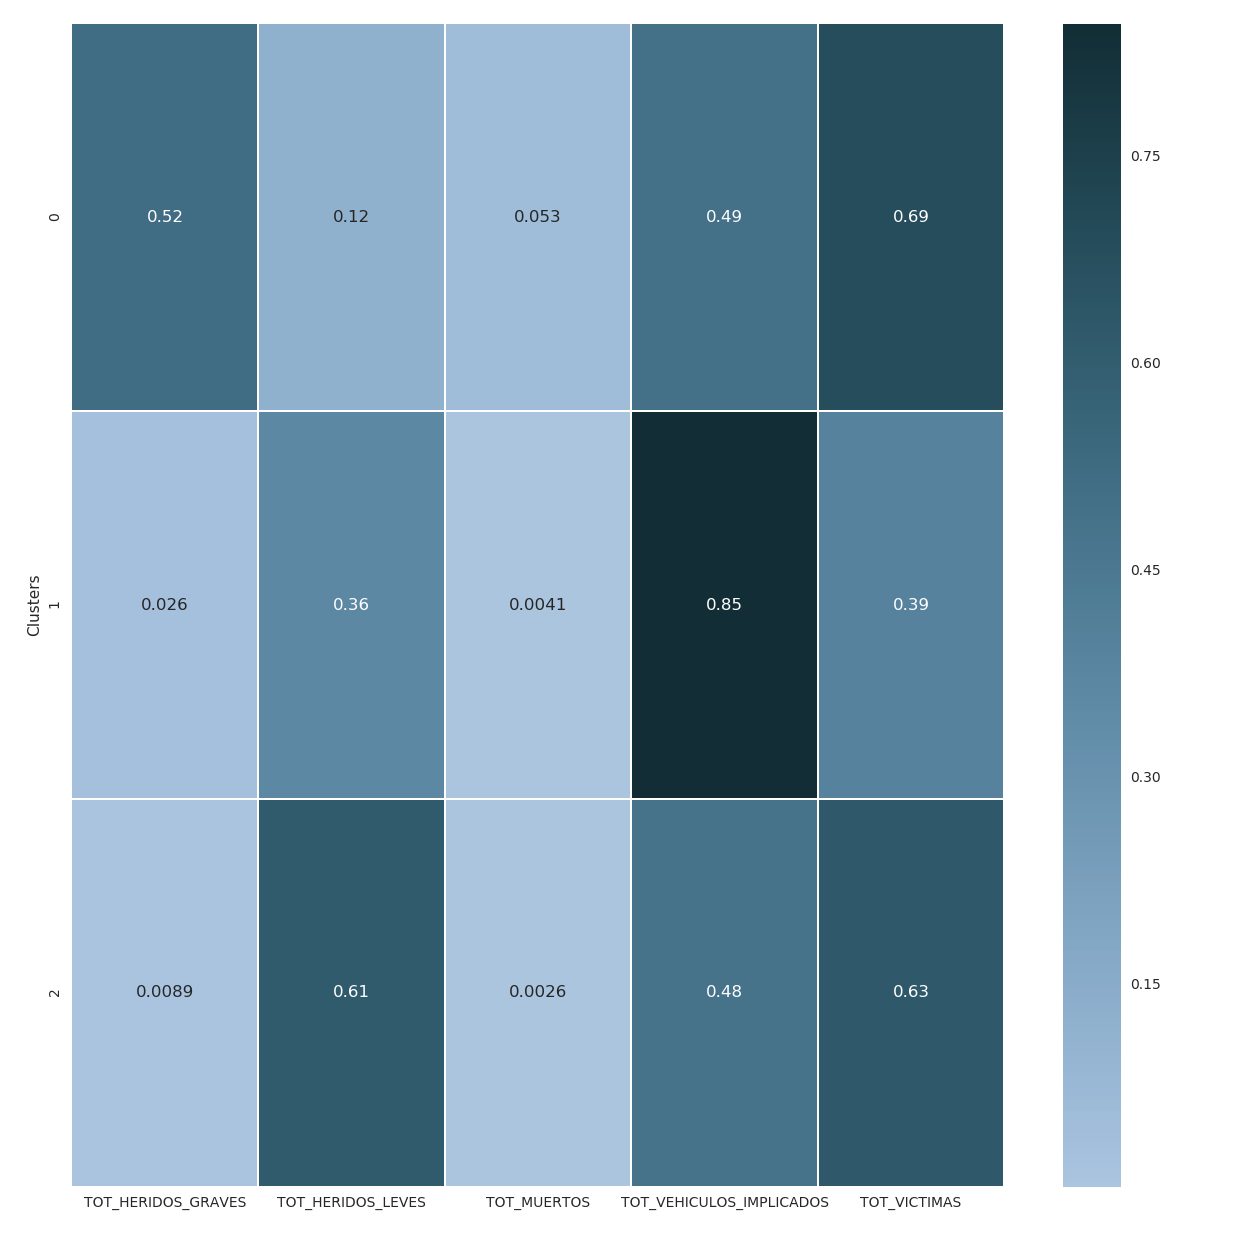
\includegraphics[scale=0.4]{heatmaps/Birch-HighwayAccidents-Heatmap.png}
		\caption{Heatmap del algoritmo Birch para el primer caso de estudio.}
	\end{figure}

	\subsection{Interpretación de la segmentación}
	En este apartado final se analizarán los resultados obtenidos basándonos en lo que se muestra en las gráficas y se intentará dar la visión más profesional posible de lo que se puede valorar de los datos recogidos.\\
	
	\subsubsection{K-Means}
	Observando la representación de la matriz de confusión, y apoyándonos en los datos de la tabla, se puede interpretar fácilmente a qué tipo de accidente se corresponde cada cluster. El cluster 0 y el cluster 2 son muy parecidos, siendo ambos accidentes donde no hay muchas víctimas graves ni fallecidos, pero sin embargo hay una gran cantidad de heridos leves, por lo que su total de víctimas asciende considerablemente. En particular, el cluster 0 recoge mayormente aquellos accidentes en los que habiendo menos vehículos se han producido más víctimas, presumiblemente por un choque más fuerte entre dos vehículos, mientras que el cluster 2 recoge los accidentes con más implicados y algo menos de víctimas. Estos datos, aparte de con la tabla de valores medios, pueden verse claramente reflejados en el heatmap del algoritmo, con la leyenda de color señalando dónde hay más víctimas y heridos leves. Adicionalmente, en la matriz de dispersión, se puede observar muy bien lo parecidos que son ambos clusters, y sin embargo cómo se pueden diferenciar, en alguna gráfica como la que representa el total de víctimas frente al total de heridos leves.\\
	
	Como la contraparte a estos dos clusters, el cluster 3 es posiblemente el más devastador, ya que representa accidentes que han tenido también bastantes víctimas pero estas han resultado heridas gravemente o han fallecido. En la matriz de dispersión puede observarse, en la intersección entre la fila y la columna que representan el total de muertos, que sin embargo hay bastantes ejemplos de este cluster que no representan accidentes mortales. No obstante, en la gráfica se aprecia que la mayor parte de todos los demás accidentes que han causado algún muerto están en el cluster 3. Además, esa misma gráfica revela un dato que teníamos como objeto de nuestro estudio: \textbf{los accidentes que suceden en autovías y autopistas no suponen víctimas mortales en la mayoría de los casos.}\\
	
	Por último, el cluster 1 representa los accidentes menos graves, con pocas víctimas y muchos vehículos implicados, como el clásico choque en cadena donde varios conductores pueden sufrir un latigazo cervical sin resultar en más complicaciones ni secuelas. Esto se puede observar de la mejor forma en la gráfica de la matriz de dispersión que representa el total de víctimas frente al total de vehículos implicados. Casi todos los accidentes en los que intervienen más de 2 ó 3 vehículos se reúnen entre el cluster 1 y el 3, sin embargo la gran diferencia existente entre ambos clusters reside en el número de víctimas, donde además en el cluster 3 la mayoría son graves. La representación en el heatmap de ambos clusters refuerza esta posición y la caracterización de estos clusters de dicha forma.
	
	\subsubsection{Birch}
	A diferencia de los clusters en los que se ha dividido anteriormente el algoritmo K-Means, este algoritmo ha reducido el número de clusters y representa esencialmente lo mismo en 3. El cluster 0 del algoritmo Birch es muy similar al agrupamiento que se encuentra en el cluster 3 del K-Means, el que tiene mayor cantidad de muertos y heridos graves. Tanto en la tabla de medias como en el heatmap se puede observar que este cluster es el que contiene los accidentes más graves, y con pocos vehículos implicados, por lo que entendemos que generalmente se trata de colisiones entre dos vehículos o de colisión frontolateral de algún vehículo con una mediana, y que generalmente han debido ser a gran velocidad para causar un impacto tan grande.\\
	
	No obstante, dicho cluster no supone una gran representación dentro del algoritmo. Si se observa la matriz de confusión de Birch se puede apreciar en distintas gráficas, entre ellas cualquiera en la que a raíz de los datos anteriores vayamos a saber que aparece este cluster, como la que representa total de muertos con el total de víctimas, que el número de puntos de la nube de puntos de la gráfica correspondientes al cluster 0 es escaso. Esto quiere decir que, o los datos están muy juntos (son muy similares), o el número de ejemplos de dicha clase es muy pequeño. A juzgar por los valores tan pequeños que tiene toda la columna de medias de muertos en el heatmap, y que el resto de clusters aparecen con una cantidad de puntos mucho mayor en cada una de las demás gráficas, considero que es un cluster que constituye pocos ejemplos.\\
	
	Es destacable que algo similar a lo que ocurre con el cluster 0 y el cluster 3 de K-Means ocurre con los clusters 1 y 2; el cluster 1 de Birch es casi un calco del cluster 1 de K-Means, y el cluster 2 de Birch lo es del cluster 0 de K-Means.\\
	
	La mejor forma de interpretar este hecho es que Birch prácticamente ha rehecho las agrupaciones de K-Means, con unas pequeñas fluctuaciones en los valores medios de cada variable debido a los cambios de asignaciones a cluster que pueda haber en las fronteras. Como podíamos observar en la tabla de resultados de los algoritmos (tabla \ref{tablaTodos1}), Birch deja un cluster sin validez al tener menos del 1\% de los datos, y este podría ser el equivalente al cluster 2 de K-Means, que era similar al cluster 0 pero con unas varianzas mayores en términos de total de vehículos implicados y de víctimas.\\
	
	Los ejemplos de Birch por tanto están clasificados siguiendo el mismo esquema que en el caso anterior, pero reducidos a un total de 3 clusters. Por la mayor diversidad que ofrece K-Means al repartir mejor sus ejemplos y por sus mejores métricas tanto Calinski-Harabaz como Silhouette, creo que es el que mejor solución obtiene de los dos, y casi aún más importante, en el que más visual e interpretativo resulta su análisis.
	
	\section{Caso de estudio 2}
	
	\subsection{¿Qué se analiza?}
	El segundo caso de estudio que se va a analizar en la práctica tiene como centro de atención los \textbf{accidentes ocurridos de madrugada}, es decir, aquellos que ocurren entre las 0:00 y las 6:00 según el criterio que he seguido. Las características que se van a tener en cuenta son las mismas que en el caso anterior, a saber, número de heridos graves y leves, número total de víctimas, número de vehículos implicados y número de muertos. De nuevo se buscará saber cómo se distribuyen principalmente los accidentes en estas horas, cuántas personas mueren o se hieren de gravedad y si representan un gran número de ejemplos o son casos que se pueden considerar aislados.\\
	
	Este caso de estudio tiene un tamaño medio. Está compuesto por 5969 ejemplos.
	
	\subsection{Resultados de los algoritmos}
	
	A continuación se muestra la tabla de los resultados de los algoritmos para este segundo caso de estudio. Como en el primer apartado, esta tabla incluirá las puntuaciones de los algoritmos según las métricas Calinski-Harabaz y Silhouette, además de los clusters en los que ha dividido los ejemplos y su tiempo de ejecución. Adicionalmente, se ha optado también por filtrar aquellos clusters que no agrupen un 1\% de los datos para que los heatmaps y tablas de medias no contengan outliers y puedan ser así más lógicos y sencillos de interpretar.
	
	\begin{table}[H]
		\centering
		\resizebox{\textwidth}{!}{
			$\begin{tabular}{ *{7}{c} }
			\toprule
			\textbf{Algorithm} & \textbf{Clusters} & \textbf{Execution time} & \textbf{CH Score} & \textbf{Silhouette Score} & \textbf{Clusters after filtering} & \textbf{Number of samples dropped}\\
			\midrule
			K-Means & 4 & 0.022 & 8773.443 & 0.78234 & 4 & 0 \\
			DBSCAN & 22 & 0.268 & 2218.602 & 0.72603 & 8 & 255 \\
			Birch & 4 & 0.183 & 4435.925 & 0.70089 & 3 & 1 \\
			Spectral Clustering & 4 & 6.952 & 7897.146 & 0.74936 & 4 & 0 \\
			Ward & 100 & 0.625 & - & - & 9 & 587 \\
			\bottomrule
			\end{tabular}$
		}
		\caption{Resultados de los algoritmos de clustering para el segundo caso de estudio.}
	\end{table}

	En este caso los resultados de los scores vuelven a ser muy similares al primer caso de estudio, pero como ya hemos trabajado con K-Means, en esta ocasión lo haremos con \textbf{Spectral Clustering}. Además, para esta ocasión contaremos también con un análisis del algoritmo \textbf{Ward}, un algoritmo de clustering jerárquico aglomerativo que genera una gran cantidad de clusters (tantos como individuos haya en la población) y los va uniendo dos a dos en cada paso, para acabar obteniendo el número de clusters indicado como parámetro. Estos dos algoritmos serán el objeto de estudio para este caso.
	
\end{document}